%% sample template file for a MSc Thesis
%% The default is with two sided setup:
\documentclass[%
oneside,    %% uncomment for onesided layout
project,    %% uncomment not thesis but project report
nosummary   %% uncomment if no summary page should be generated
]{USN-MSc}

% The following command removes the chapter names form the header
% (comment/remove) if you prefer to have them:
\pagestyle{plain}

% --- Bibliography setup ---
%%% default is the "ieee" style
\usepackage[style=ieee, sorting=none]{biblatex}
%%% If you want to use "author-year" style
%%% where `\cite{Foo2011}` generates "Foo et al. (2011)"
%%% and   `\parencite{Foo2011}` generates "(Foo et al. 2011)"
%%% then comment the line above and use
%\usepackage[style=authoryear]{biblatex}
%%% or
%%% if you want to use "alphabetic" style then use
%%% where `cite[Foo2011]` generates "[Foo11]"
%%% then comment the line above and use
%\usepackage[style=alphabetic]{biblatex}
%%% instead.
%% load the bib file:
\addbibresource{MScThesis.bib}

\usepackage{lipsum} % just for providing fill text used in this template
\usepackage{array} % for adjusting tables?

% --- general setup ---
%% Please fill in the following parameters:
\newcommand{\mytitle}{%
%% title:
Assignments for section 1 (W1.2-W1.6)
}

\newcommand{\mysubtitle}{%
%% master programme (for thesis only)
%% uncomment the appropriate one:
%%Electrical Power Engineering
%Energy and Environmental Technology
%Industrial IT and Automation
%Process Technology
}

\newcommand{\mykeywords}{%
%% keywords (for thesis only):
<keyword one, keyword two, \ldots>
}

\newcommand{\myauthor}{%
%% author(thesis) or group code (project):
223786 Lars Rikard Rådstoga
}

\newcommand{\myparticipants}{
%% group participants (for project only)
<First participant>\\
<Second participant>\\
<Third participant>\\
<Fourth participant>
}

\newcommand{\supervisor}{%
%% supervisor:
<Supervisor's Name>}

\begin{document}

% --- title page setup ---
%\USNtitlepage%
%%% Please provide the following information:
%%% #1 optional figure (set to {} if not wanted)
%{%
%  {\normalsize}
%  \begin{figure}[!ht]
%    \centering
%   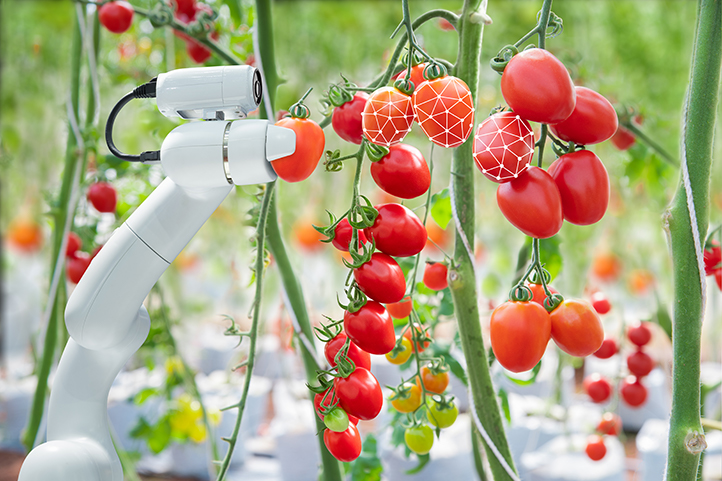
\includegraphics[width=0.8\textwidth]{TomatoPickerBot}
%   \label{fig:tomatoBot}
% \end{figure}
%}
% --- title page setup ---
\USNtitlepage%
%% Please provide the following information:
%% #1 optional figure (set to {} if not wanted)
{%
  {\normalsize}
   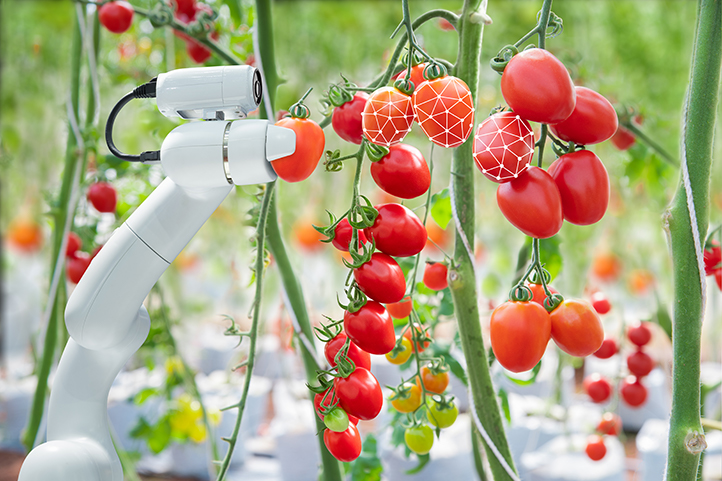
\includegraphics[width=\textwidth]{TomatoPickerBot}}
%% #2 Project partner:
{<Project partner>}
%% #3 Summary:
{%
\lipsum[6-7]
}


%\chapter*{Preface}
%\label{ch:preface}
%\addcontentsline{toc}{chapter}{Preface}
%\lipsum[1-3]
%\bigskip
%Porsgrunn, \today

%\myauthor %% for thesis
%\myparticipants %% for project


%% table of contents
\tableofcontents
\addcontentsline{toc}{chapter}{\contentsname}

%\listoffigures % out-comment if unwanted
%\addcontentsline{toc}{section}{\listfigurename}

%\listoftables  % out-comment if unwanted
%\addcontentsline{toc}{section}{\listtablename}



\chapter{Definition of autonomous systems}
\label{ch:definition}
The following chapter displays different definitions of the phrase "autonomous system".
\section{Definitions}
There are many degrees of definitions for the phrase "autonomous system", which vary in levels of abstraction. 
As to not repeat the dictionary definitions given in the lectures, I decided to firstly ask the first "AI chatbot" I could find on Google, see Figure \ref{fig:chat-bot}
\begin{figure}[!ht]
  \centering
  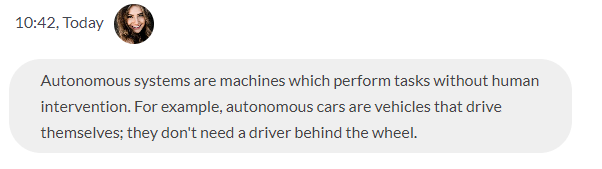
\includegraphics[width=0.8\textwidth]{AutonomousSystemChatBotDefinition}
  \caption{An AI chatbot's response to the request of defining the phrase "autonomous system" \cite{ChaiChat90:online}.}
  \label{fig:chat-bot}
\end{figure}
This is close to the exact same definition that can be found in the textbook "Introduction to AI Robotics":
"Function autonomously" indicates that the robot can operate, self-contained, under all reasonable conditions without requiring recourse to a human operator 
\cite{murphy2000introduction}.
A third, very technical definition was found in "Autonomous Systems - An Architectural Characterization" and can be paraphrased \cite{Sifakis}:
An autonomous system consists of both an agent and a system, the agent contains modules dealing with the fundamental aspects of autonomy.
These modules are perception, refection, goal management, planning and self-adaptation. How well these features are coordinated relates to how well an agent performs in pursuing its goal.
And the system relates to sensors and actuators which the agent has to use and operate to perceive its environment and calculate its control strategy.

\section{My definition}
\label{sec:myDefinition}
A definition of an autonomous system could be:
An intelligent system: must be equipped with sensors for perceiving its own and its objectives' positions; 
have the ability to classify objectives, paths and obstacles; 
and be able to calculate optimal paths and actions to maximize its chances of success;
in case of failure the system should independently try to correct the error.

\section{Explanation}
\label{sec:myExplanation}
My system is supposed to pick fruit and be an unmanned ground vehicle.
So, the definition fits well in the following sense:
It has to know where it is positioned, where obstacles are and where the path to its objectives (fruit) is.
It has to tell ripe fruit from unripe and rotten, it should also know what a clear path looks like.
It needs to be able to control its actuators in an orderly fashion to move between bushes, loading stations, etc. 
And it has to move arms and claws or such to pick fruit. All without damaging bushes, people, itself, other fruit and more.

\chapter{System Diagrams}
\label{ch:diagrams}
The following chapter contain diagrams meant to contextualize the system.

\section{Nine window diagram}
\label{sec:nineWindow}
The nine window diagram describes the past, present, and future state of the system, its sub-systems and its user, see table \ref{tab:nineWindow}.
\begin{table}[!ht]
  \caption{Nine window diagram}
   \centering
    \begin{tabular}{ | m{3cm} | m{3cm} | m{3cm} | m{5cm} |}
     \hline
     Perspective & Past & Present & Future \\ \hline
     Super system & Farmer or group of farmers. & Farmer or group of farmers. 
     & Small scale groups for urban farming or small farms. \\ \hline
     System & Cheap labor harvesting by hand. & Autonomous harvester. 
     & Autonomous multipurpose robot for pollinating, weeding, trimming, manuring and more. \\ \hline
     Sub-system & Propulsion, navigation. & Propulsion, navigation, classification, collection, logistics. 
     & Tool or mode change, learning, weather/climate regulated. \\ \hline
     \end{tabular}
     \label{tab:nineWindow}
 \end{table}

\section{Cartoon}
\label{sec:cartoon}

Figure \ref{fig:cartoon} displays a rough start to finish cycle of the system, some tasks described will happen multiple times.

\begin{figure}[!ht]
  \centering
  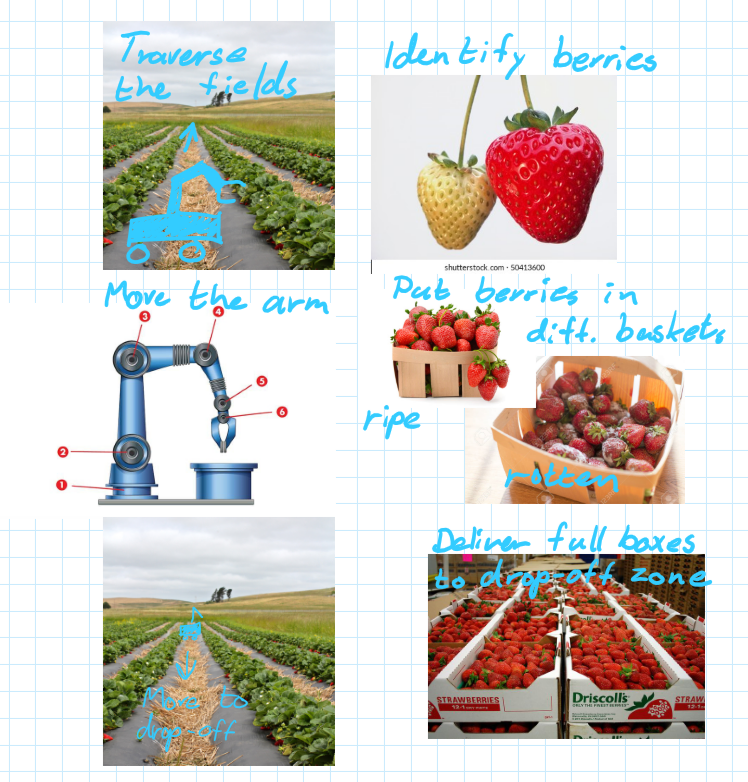
\includegraphics[width=0.8\textwidth]{Cartoon}
  \caption{A quick sketch visualizing the system functions.}
  \label{fig:cartoon}
\end{figure}

\section{Context diagram}
\label{sec:contextDiagram}

Figure \ref{fig:contextDiagram} is a context diagram that displays elements involved in the system.

\begin{figure}[!ht]
  \centering
 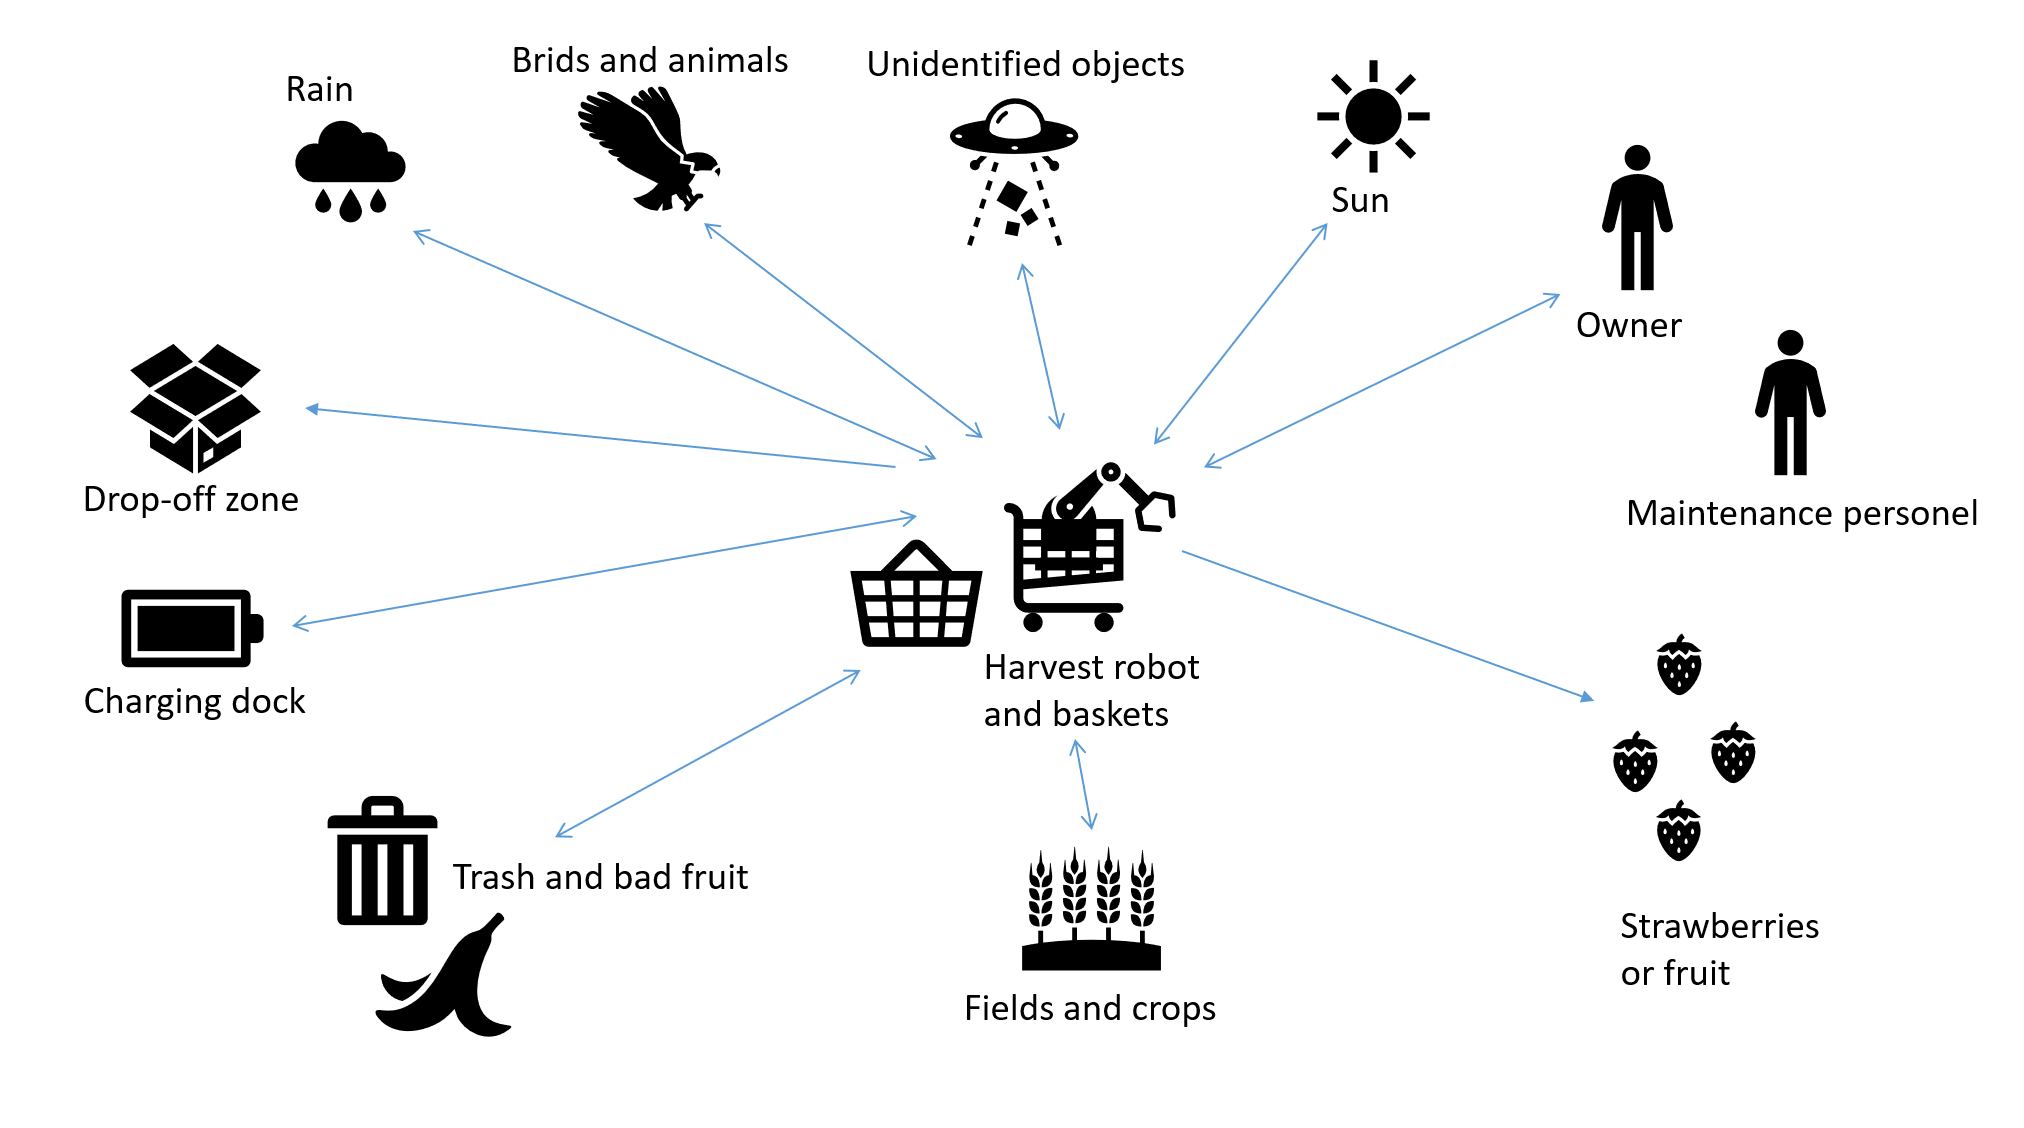
\includegraphics[width=0.8\textwidth]{ContextDiagram}
 \caption{Context diagram of the system.}
 \label{fig:contextDiagram}
\end{figure}

\section{IDEF0 (of the main function)}
\label{sec:IDEF0}

The diagram in \ref{fig:idef0} describes the input (left), control (top), resources (bottom), and output (right) of the main system function.

\begin{figure}[!ht]
  \centering
 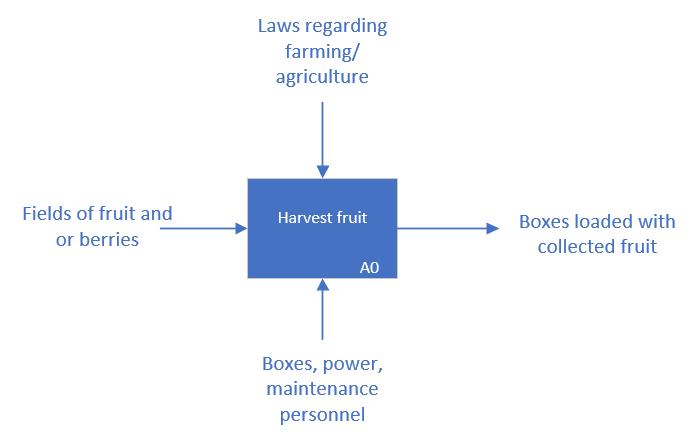
\includegraphics[width=0.8\textwidth]{IDEF0}
 \caption{Model of the main function for the system.}
 \label{fig:idef0}
\end{figure}

\chapter{Impact on society}
\label{ch:impact}

Automation is clearly impacting our society, it affects our efficiency in various work and everyday life.
But are the effects of automation only positive? The answer to this question is most definitely no.
Most effects are probably positive and some are negative, which is the way of the analog world.
For many of us, automation means that we could get more time to do what we truly want.
For others, it could mean that their profession as assembly line workers, lawn mowers, or perhaps truck drivers become redundant.
However, it is argued that automation also create new jobs \cite{CERNETIC2002167}.
And the current unemployment rates as of the summer of 2022 are record low in countries like Norway \cite{Lavestea6:online} and the USA \cite{Theunemp77:online}.
This isn't conclusive evidence that automation affects the job market in either a positive or negative way.
Other actors might be stimulating the job market to compensate for disappearing jobs.
With growing efficiency in the workplace, because of automation, digitalization, and more, people get more work done in less time.
On the other hand, worse paid jobs will either require increased subsidization to viably supply competing living wages.
Some jobs, such as teaching and nursing, are hard to fully automate, and it is probably strongly argued in favor of protecting the human factor in those professions.
Thus, those professions require more funding. On another note, 
fields like seasonal fruit and berry harvesting doesn't pay well enough,
in countries like Norway, to attract local workers anymore, 
which is reported in media, year after year \cite{Toavtrej43:online}.
If anything shift of jobs is a result of the free market, capitalism, rather than evil innovations.

Other interesting questions regarding automation's impact on society are:
Do we lose our humanity when we do less manual labor?
How is the less gifted affected by increasing requirements in the job market, when simpler jobs are disappearing?


%Removing jobs, what should people do now?
%Are we losing our humanity?
%In accident scenarios involving autonomous robots, 
%how should the robot prioritize? 
%Should it be a true utilitarian, should it comply with the common consensus, 
%should it make human mistakes on purpose,
%or should it be decisions be normally distributed?

\begin{figure}[!ht]
   \centering
  \includegraphics[width=0.8\textwidth]{USN_logo}
  \caption{Diagram of influences on the system.}
  \label{fig:diagramInfluences}
\end{figure}


\chapter{Legal and ethical aspects}
\label{ch:legal}
The following chapter contains a brief discussion on legal and ethical aspects of automation and autonomy.

\section{Discussion}
\label{sec:legalEthicalAspects}

Most things are dangerous in the hands of people with evil intentions. Knives are useful in the kitchen,
but they can also be murder weapons. Everybody needs water to survive, but floods can destroy houses and people can die of drowning.
The same goes for technology, AI, and autonomy\dots

It is easy to think that the harvester robot will operate in such a safe and open environment that there won't be many or any legal difficulties.
As with ethical aspects, there might be some aspects where decisions made by the system might be classified as ethically good or bad,
but the design of the robot should be of such caliber that physical harm should be hard for the robot to inflict. 
A steady paced and carefully moving robot could be both advantageous for energy efficiency and for humans or animals coming into contact with the robot.

Gentle logic could also be implemented meaning it shouldn't fight unexpected resistance. 
So if it experiences unexpected behavior: e.g. the claw doesn't close properly, or it encounters an undetected blockade.
Then it shouldn't use strength to solve the issue, but rather take a step back and re-analyze.

A small scale robot, say a 10 to 30 kg build, and with a weak motor for the claw, might not have much power that can be used for destruction. 
But in case of accidents, two points need to be considered: 
\begin{enumerate}
  \item Predetermined ethical decision priorities.
  \item Logging decision reasonings.
\end{enumerate}

IEEE are working on a series of standards, the P7000-series, to promote ethics in AI \cite{7924235}. 
The P7001 standard aims to promote transparency and says that decisions made by an autonomous robot should always be traceable. There isn't much of a downside to this, other than requiring slightly more data storage space. It might be a difficult task to translate an AIs decision language into something humans can interpret, especially if the computer relies on one or multiple machine learning models. However, not an impossible task and decision logs can also be very useful to fine-tune main functions of a system.

Predetermined ethical decision prioritization means that generally computers are much quicker at making split-second decisions and computers are deterministic machines. Thus, it will most of the time be possible to fairly decide what to do in a dangerous situation. But what ethics should be practiced in these situations? Should it be purely utilitarian, should a probability model of ethics based on peoples response to numerous trolley-problem dilemmas be used, or should the programmer decide? Truly a difficult question, which should be studied and argued hard in order to answer. But there should be a distinction of strictness of responsibility to this problem depending on a multitude of factors, such as: Should it be used by the common man, e.g. a car? Should it be used in private, closed environments? Should it be operated or managed by trained workers? As the fruit-picker should operate inside a private area, i.e. a farm, it should not be enforced as strict as in other arenas, but still highly recommended for future-proofing and fine-tuning.

\chapter{Human interaction(s) of your autonomous system}
\label{ch:human}
The following chapter contains a brief discussion on human interaction with automated systems.
\section{Human-automation interaction issues}
\label{sec:humanAutomationIssues}
A classic problem with human-automation interaction is out-of-loop operators. The system is automated to such a degree that it requires very little attention of the operator during a regular operating state. However, this leads to two factors: firstly, operators get less familiar with the system and less practice operating it manually. Secondly, operators will pay less attention to the system and its surroundings. Both factors resulting in less "situational awareness" for the operator \cite{Gruhn2011HumanMI}. However, this fruit-picker does not carry out as big of a risk during operation compared to oil refinery plants or driving in a car. Think of the fruit-picker like a robotic vacuum or lawn mower, its main purpose is to carry out a boring, repetitive task that is nevertheless low-risk. The worst that should be able to happen if it unexpectedly bugs out and stops working is that a few berries are damaged. And in case of mass failure of multiple units, there will be a problem harvesting in time. \cite{NozzleWi94:online}
\section{Issues related to level of automation}
\label{sec:issuesLevelAutomation}
In an array of systems it is advantageous to implement a degree of automation if it isn't already. According to Endsley \cite{article}, there are five levels of automation: none, decision support, consensual AI, monitored AI and full automation. The different levels display varying dependence on human and machine as seen in \ref{fig:levelsOfAuto}.

\begin{figure}[!ht]
  \centering
  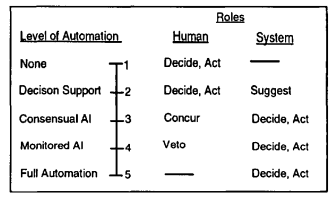
\includegraphics[width=0.8\textwidth]{LevelsOfAutonomy}
  \caption{Table explaining varying levels of control \cite{article}.}
  \label{fig:levelsOfAuto}
\end{figure}

Furthermore, Endsley \cite{article} explores the situational awareness and the decision time of groups performing high-level cognitive tasks: each group aided differently according to the aforementioned levels of automation. Each group solved four tasks with the aid they were assigned, followed up by doing the tasks twice in an "automation failure" scenario. All groups trended towards faster completion times during the four initial tasks and when switched to "automation failure" scenario the first decision always took longer than the second. The difference between first and second completion time in the "failure" scenario is probably explained as a mixture of panic, situational awareness, and training. And, perhaps because of a lack of training, the groups that was helped by the higher degrees of automation used the longest to solve tasks in manual mode after failure. Also, the decrease in decision time between the first and second failure tasks signifies a lack of situation awareness. Another thing that is worth noticing is the fact that the manual and low-level automation groups performed best before and after the failure in terms of decision time. This is important knowledge when designing systems around high-risk systems such as plane autopilots.

\section{Potential threats and opportunities}
\label{sec:threatsOpportunities}

Numerous threats are present in any system, and the design of the system should take these into consideration. The goal of the fruit-picker robot is to operate in the 4th degree of automation: monitored AI. Combining machine learning techniques such as classification and reinforcement learning. Classification should be used to tell ripe from unripe berries. Reinforcement learning should be used to 

% A dummy command that causes all bibliographyentries to be displayed
% even though there were not cited in the document. Used for demonstration
% purposes only in this template file.
~\nocite{*}

\cleardoublepage

% The bibliography should be displayed here...
%\printbibliography[heading=bibintoc]
% You rather like to call the bibliography "References"? Then use this instead:
\printbibliography[heading=bibintoc, title={References}]


%\appendix
%\renewcommand{\appendixname}{Paper} %% So we get 'Paper X' displayed instead


%\chapter[Short Title of Paper A]{Title of Paper A (probably very long and therefore not good to have in the header)}
%\label{paper-a}
%
%\paragraph{Note}
%Since some papers tend to have a rather long title it is good to provide the optional short title which then will be displayed in the table of contents and header instead of the long original title.
%On the openening page of the chapter the orginal \emph{long} title will be displayed.\bigskip
%
%\emph{Short descriptive text of paper follows here.}\bigskip
%
%The paper itself needs to be included in the published form as PDF on the next pages.
%This can be done using the \texttt{pdfpages} package by adding the command:
%
%\begin{verbatim}
%\includepdf{pages=-,openright}{Filename}
%\end{verbatim}
%
%You can omit the \texttt{.pdf} when specifying the \texttt{Filename}. Also you should include always include the option \texttt{openright} since it would look strange to have the paper starting at the back of the cover page.
%
%There are more options like only adding specific pages:
%\begin{verbatim}
%\includepdf{pages=2-6,openright}{Filename.pdf}
%\end{verbatim}

%For more options see Appendix~\ref{paper-b} where the most important pages of the \texttt{pdfpages} manual were inlcuded using \texttt{pdfpages}.


%%% Command to include a PDF file directly including all pages:


%\chapter[Short Title of Paper B]{Title of Paper B}
%\label{paper-b}
%Short descriptive text of paper follows here.
%
%Here we included the first five pages of the \texttt{pdfpages} manual itself.
%
%\includepdf[pages=1-5,openright]{fig/pdfpages}
%
\end{document}

%%% Local Variables:
%%% mode: latex
%%% TeX-master: t
%%% End:
